
\section{Data-Centric Workflows}\label{sec:dataCentricWorkflows}

Consider a Friend Finder application in which multiple users carry mobile devices that periodically transmit their location. Assume that they have agreed to share some of their personal information. A user in this scenario may want to \textit{Find friends recently located no more than 3 km away from me, which are over 21 years old and that are interested in art}.

Data services produce data in one of two ways: on-demand in response to a given request, or continuously as a data stream. In either case, the data service exposes an interface, composed of several operations and supported by standardized protocols. The JavaScript Object Notation is used to represent the data. Accordingly, objects are built from atomic values, nested tuples, and lists.

For instance, in our scenario the users' location is available by a stream data service with the interface
	
$\mathtt{subscribe() \rightarrow \lceil location:\langle nickname, coor\rangle\rceil}$
	
\noindent consisting of a subscription operation that after invocation will produce a stream of location tuples, each with a nickname that identifies the user and his/her coordinates. The rest of the data is produced by the next two on-demand data services, each represented by a single operation
	
$\mathtt{profile(nickname) \rightarrow person:\langle age, sex, email\rangle}$
\\
\hspace*{0.50cm}$\mathtt{interests(nickname) \rightarrow \left[s\_tag:\langle tag, score\rangle\right]}$

The first provides a single person tuple denoting a profile of the user, once given a request represented by her nickname. The second produces, given the nickname as well, a list of s\_tag tuples denoting the interests of the user by scored tags (\eg{} 'music' with 8.5).
	
In order to obtain the desired result we need to give to it an executable form, in our case a workflow of activities implementing a service coordination. Workflows are built by the parallel and sequential composition of activities that are bound to data and computation services; the first provide the data, while the latter process them as required.

\subsection{Workflow Model}\label{subsec:workflowModel}

The workflow is specified as an Abstract State Machine (ASM) \cite{Gurevich:1995:EAL:233976.233979}, which can be represented as a series-parallel graph. The ASM specification of the service coordination corresponding to our example application is presented in Listing \ref{WorkflowListing}, while its workflow representation is given in Figure \ref{fig:servCoorExample}. It includes the location, profile, and interests data services, as well as computation services for various relational operations such as selections, joins, and a time-based window bounding the location stream to recent data (e.g. location notifications obtained within the last 10 minutes).

\lstdefinelanguage{AbStM}[]{Pascal}{
   morekeywords={seq, endseq, iterate, skip, par, endpar},
}

\lstset{language=AbStM,showstringspaces=false}
\begin{lstlisting}[caption={ASM specification for example application},label=WorkflowListing]
seq
   par
      seq
         par
            seq
               location := l.location()
               locWin := comp.timeWin(location,10)
	             distSel := comp.funCallSel(locWin, 
	              d.dist(lat,lon,48.85,2.29)<3.0 )
            endseq
            profile := profile.profile()
         endpar
         lp := comp.bindJoin(distSel,profile,nickname=nickname)
         ageSel := comp.selection(lp,age > 21)
      endseq
      interests := i.interests()
   endpar
   lip := comp.bindJoin(lp,interests,nickname=nickname)
   tagSel := comp.selection(lip,tag='art')
   output := comp.output(tagSel)
endseq
\end{lstlisting}

\begin{figure}
	\centering
		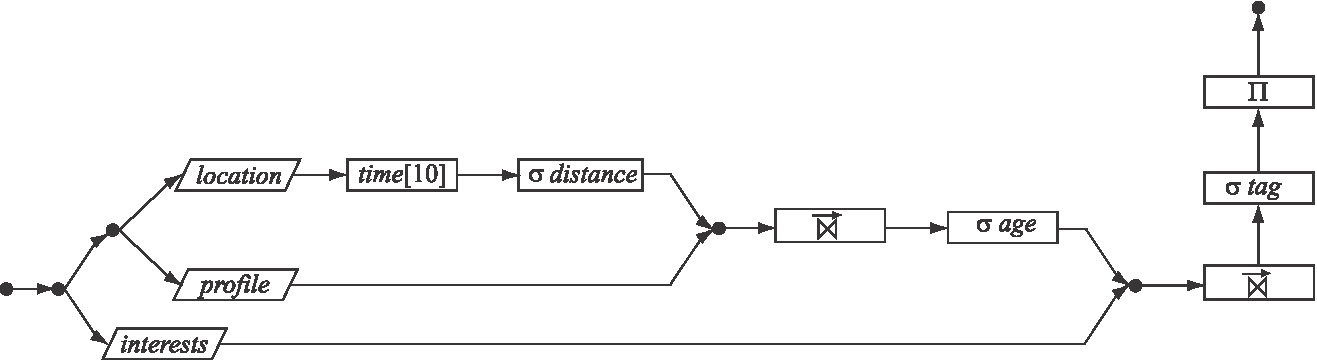
\epsfig{file=Images/FriendFinderQueryWF.pdf, scale=0.50}
		\caption{Data-centric workflow for example application}
		\label{fig:servCoorExample}
\end{figure}

A workflow $W$ is modeled as a directed acyclic graph $W=(V, E, in, out, A, C)$ where:
		\begin{center}
			\footnotesize
			\begin{tabular}{rp{7.5cm}}
				$V$                      & is a set of vertices \\
				$E \subseteq V \times V$ & is a set of edges \\
				$A \subseteq V$          & is a set of activities \\
				$\{in, out\} \subseteq A$     & are the initial and final activities of $W$\\
				$C \subseteq V$          & is a set of composition operators $\{par_1,...,par_n\}$\\.     
			\end{tabular}   
		\end{center}
There are three types of vertices: \textit{activities} perform a service method invocation and always have ancestor and descendant vertices, \textit{in} vertices have no ancestors and their only goal is to launch the first \textit{activity} of the workflow, \textit{out} vertices have no descendants and stop the workflow execution after the last \textit{activity}. A series of construction rules enable to generate a workflow graph from a given ASM, which are detailed in \cite{vcv}.

\subsection{Computation services}\label{subsec:computationServices}

Two kinds of computation services form part of our approach: simple computation services and composite computation services specified in the ASASEL language.

%\begin{figure*}
%   \begin{center}
%      \scalebox{0.785}{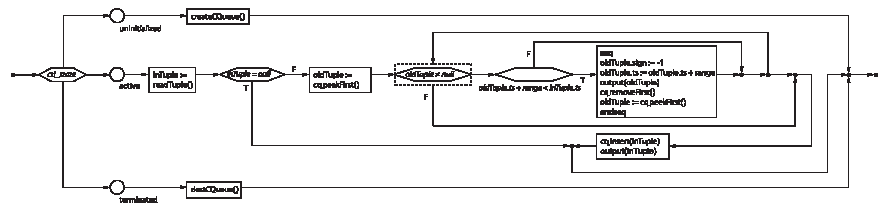
\includegraphics[natwidth=12.31cm,natheight=7.16cm]{Images/time-based-window.pdf}}
%   \end{center}
%   \caption{Workflow representation of the time-based window}
%   \label{fig:timeBasedWindowWF}
%\end{figure*}

\textbf{Simple computation services}  involve a single service operation invocation to process data. For instance, a distance computation service that relies on a \texttt{geo-distance} service, which provides the capability to calculate the geographical distance between two points, e.g., by Vincenty's formula.

\textbf{Composite computation services}  process data by multiple operation invocations, possibly from different services, and often also by the manipulation of local data. These tasks are organized in a service coordination specified in the ASASEL language and represented as a workflow, following a model in which we add data items as well as conditional and iteration constructs to our basic parallel and sequential composition workflow model illustrated in Figure \ref{fig:servCoorExample}.
		
The specification of a time-based window composite service in ASASEL is presented in Listing \ref{TimeWindowListing}, based on a simple \texttt{calendar-queue} service. It has a corresponding workflow representation as detailed in \cite{vcv}.
		
\lstset{language=AbStM,showstringspaces=false}
\begin{lstlisting}[caption={ASM specification for the time-based window},label=TimeWindowListing]
if( ctl_state = 'active')
  seq
     inTuple := readTuple()
     if(inTuple = nil)
        skip
     else
        seq
           oldTuple := cq.peekFirst()
           iterate(oldTuple != nil)
              if(oldTuple.ts + range < inTuple.ts)
                 seq
                    oldTuple.sign := -1
                    oldTuple.ts := oldTuple.ts + range
                    output(oldTuple)
                    cq.removeFirst()
                    oldTuple := cq.peekFirst()
                 endseq
           pq.enqueue(inTuple)
           output(inTuple)
        endseq
  endseq
\end{lstlisting}







		










